\documentclass[1p]{elsarticle_modified}
%\bibliographystyle{elsarticle-num}

%\usepackage[colorlinks]{hyperref}
%\usepackage{abbrmath_seonhwa} %\Abb, \Ascr, \Acal ,\Abf, \Afrak
\usepackage{amsfonts}
\usepackage{amssymb}
\usepackage{amsmath}
\usepackage{amsthm}
\usepackage{scalefnt}
\usepackage{amsbsy}
\usepackage{kotex}
\usepackage{caption}
\usepackage{subfig}
\usepackage{color}
\usepackage{graphicx}
\usepackage{xcolor} %% white, black, red, green, blue, cyan, magenta, yellow
\usepackage{float}
\usepackage{setspace}
\usepackage{hyperref}

\usepackage{tikz}
\usetikzlibrary{arrows}

\usepackage{multirow}
\usepackage{array} % fixed length table
\usepackage{hhline}

%%%%%%%%%%%%%%%%%%%%%
\makeatletter
\renewcommand*\env@matrix[1][\arraystretch]{%
	\edef\arraystretch{#1}%
	\hskip -\arraycolsep
	\let\@ifnextchar\new@ifnextchar
	\array{*\c@MaxMatrixCols c}}
\makeatother %https://tex.stackexchange.com/questions/14071/how-can-i-increase-the-line-spacing-in-a-matrix
%%%%%%%%%%%%%%%

\usepackage[normalem]{ulem}

\newcommand{\msout}[1]{\ifmmode\text{\sout{\ensuremath{#1}}}\else\sout{#1}\fi}
%SOURCE: \msout is \stkout macro in https://tex.stackexchange.com/questions/20609/strikeout-in-math-mode

\newcommand{\cancel}[1]{
	\ifmmode
	{\color{red}\msout{#1}}
	\else
	{\color{red}\sout{#1}}
	\fi
}

\newcommand{\add}[1]{
	{\color{blue}\uwave{#1}}
}

\newcommand{\replace}[2]{
	\ifmmode
	{\color{red}\msout{#1}}{\color{blue}\uwave{#2}}
	\else
	{\color{red}\sout{#1}}{\color{blue}\uwave{#2}}
	\fi
}

\newcommand{\Sol}{\mathcal{S}} %segment
\newcommand{\D}{D} %diagram
\newcommand{\A}{\mathcal{A}} %arc


%%%%%%%%%%%%%%%%%%%%%%%%%%%%%5 test

\def\sl{\operatorname{\textup{SL}}(2,\Cbb)}
\def\psl{\operatorname{\textup{PSL}}(2,\Cbb)}
\def\quan{\mkern 1mu \triangleright \mkern 1mu}

\theoremstyle{definition}
\newtheorem{thm}{Theorem}[section]
\newtheorem{prop}[thm]{Proposition}
\newtheorem{lem}[thm]{Lemma}
\newtheorem{ques}[thm]{Question}
\newtheorem{cor}[thm]{Corollary}
\newtheorem{defn}[thm]{Definition}
\newtheorem{exam}[thm]{Example}
\newtheorem{rmk}[thm]{Remark}
\newtheorem{alg}[thm]{Algorithm}

\newcommand{\I}{\sqrt{-1}}
\begin{document}

%\begin{frontmatter}
%
%\title{Boundary parabolic representations of knots up to 8 crossings}
%
%%% Group authors per affiliation:
%\author{Yunhi Cho} 
%\address{Department of Mathematics, University of Seoul, Seoul, Korea}
%\ead{yhcho@uos.ac.kr}
%
%
%\author{Seonhwa Kim} %\fnref{s_kim}}
%\address{Center for Geometry and Physics, Institute for Basic Science, Pohang, 37673, Korea}
%\ead{ryeona17@ibs.re.kr}
%
%\author{Hyuk Kim}
%\address{Department of Mathematical Sciences, Seoul National University, Seoul 08826, Korea}
%\ead{hyukkim@snu.ac.kr}
%
%\author{Seokbeom Yoon}
%\address{Department of Mathematical Sciences, Seoul National University, Seoul, 08826,  Korea}
%\ead{sbyoon15@snu.ac.kr}
%
%\begin{abstract}
%We find all boundary parabolic representation of knots up to 8 crossings.
%
%\end{abstract}
%\begin{keyword}
%    \MSC[2010] 57M25 
%\end{keyword}
%
%\end{frontmatter}

%\linenumbers
%\tableofcontents
%
\newcommand\colored[1]{\textcolor{white}{\rule[-0.35ex]{0.8em}{1.4ex}}\kern-0.8em\color{red} #1}%
%\newcommand\colored[1]{\textcolor{white}{ #1}\kern-2.17ex	\textcolor{white}{ #1}\kern-1.81ex	\textcolor{white}{ #1}\kern-2.15ex\color{red}#1	}

{\Large $\underline{12n_{0514}~(K12n_{0514})}$}

\setlength{\tabcolsep}{10pt}
\renewcommand{\arraystretch}{1.6}
\vspace{1cm}\begin{tabular}{m{100pt}>{\centering\arraybackslash}m{274pt}}
\multirow{5}{120pt}{
	\centering
	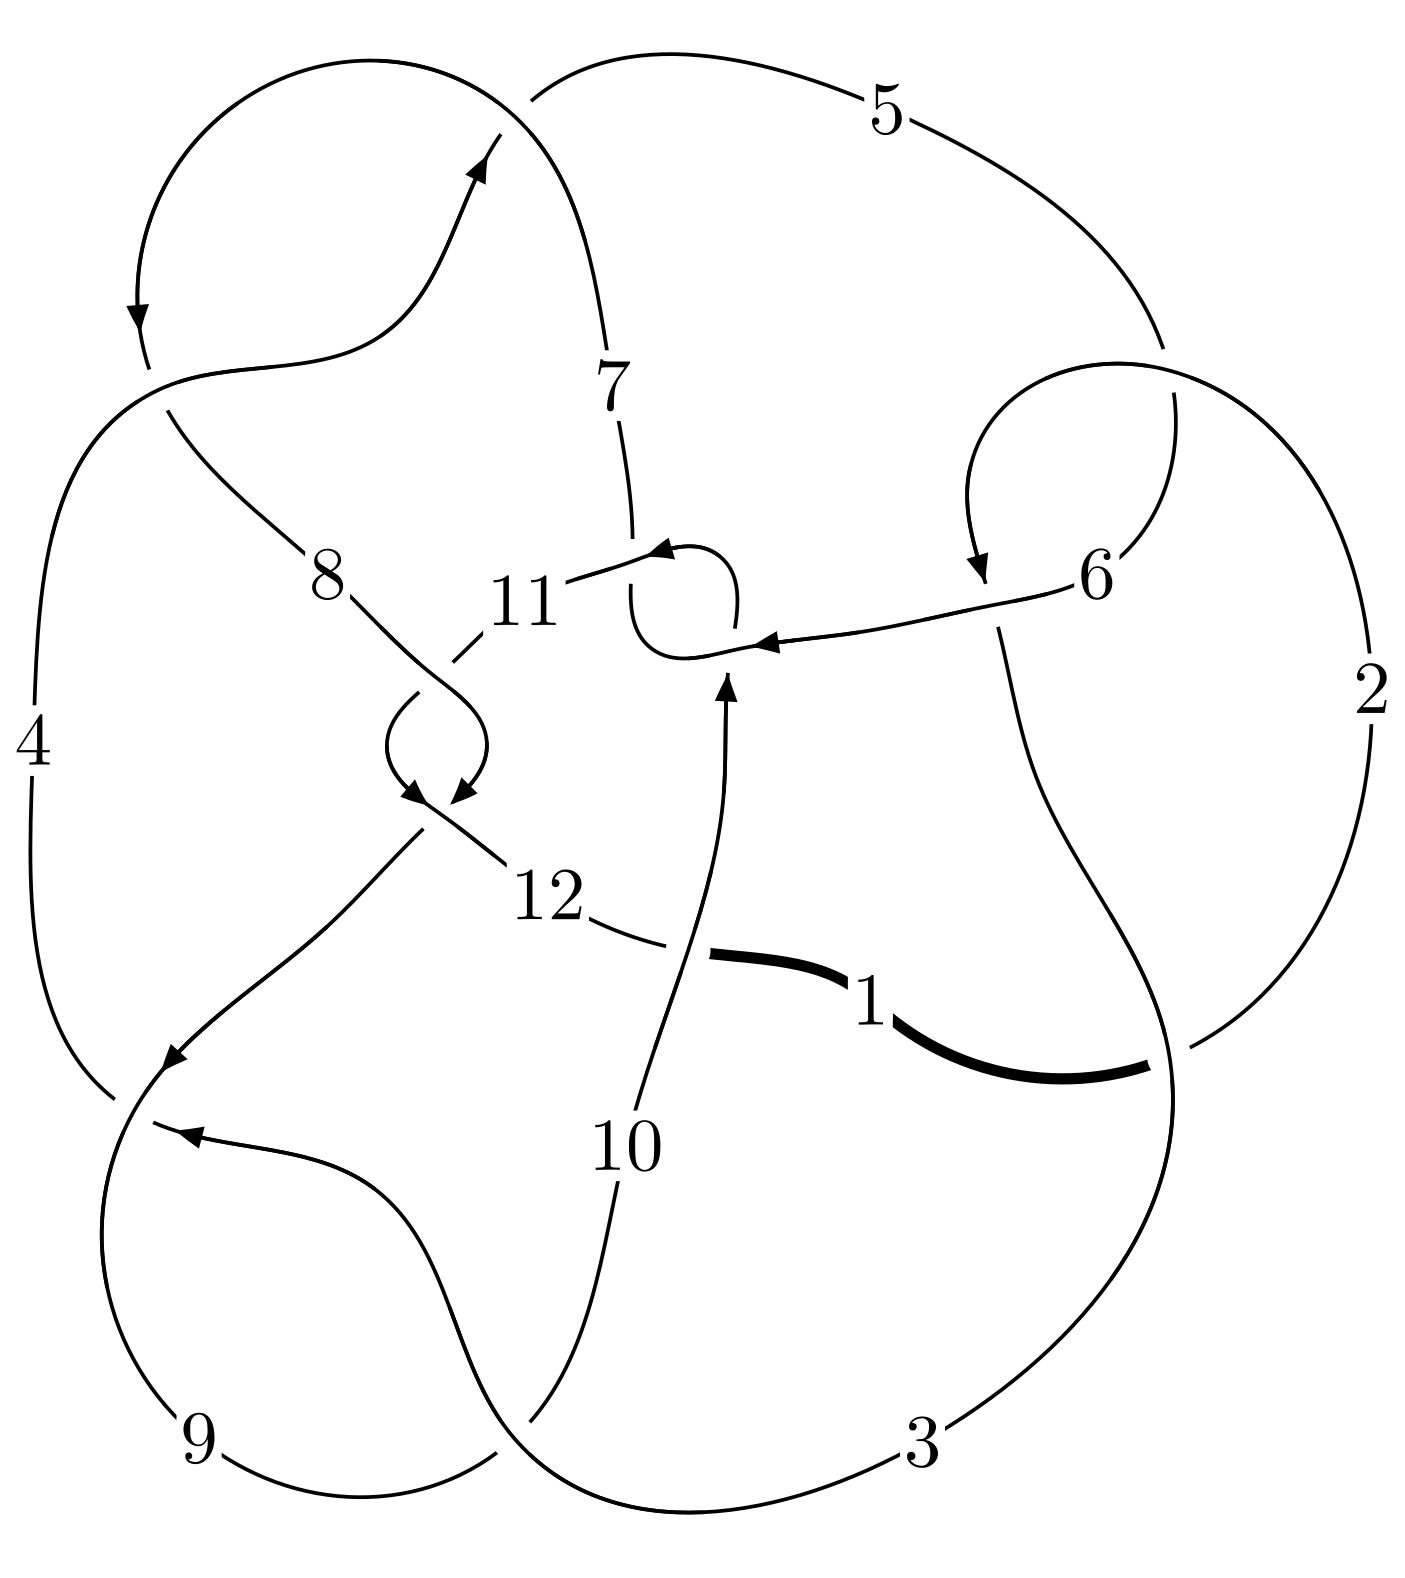
\includegraphics[width=112pt]{../../../GIT/diagram.site/Diagrams/png/2603_12n_0514.png}\\
\ \ \ A knot diagram\footnotemark}&
\allowdisplaybreaks
\textbf{Linearized knot diagam} \\
\cline{2-2}
 &
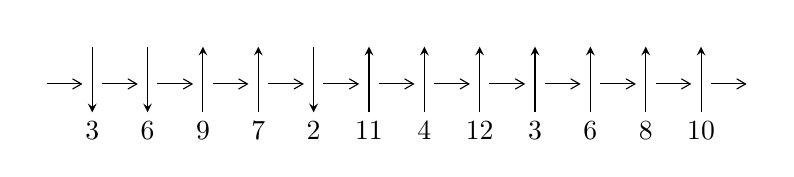
\begin{tikzpicture}[x=20pt, y=17pt]
	% nodes
	\node (C0) at (0, 0) {};
	\node (C1) at (1, 0) {};
	\node (C1U) at (1, +1) {};
	\node (C1D) at (1, -1) {3};

	\node (C2) at (2, 0) {};
	\node (C2U) at (2, +1) {};
	\node (C2D) at (2, -1) {6};

	\node (C3) at (3, 0) {};
	\node (C3U) at (3, +1) {};
	\node (C3D) at (3, -1) {9};

	\node (C4) at (4, 0) {};
	\node (C4U) at (4, +1) {};
	\node (C4D) at (4, -1) {7};

	\node (C5) at (5, 0) {};
	\node (C5U) at (5, +1) {};
	\node (C5D) at (5, -1) {2};

	\node (C6) at (6, 0) {};
	\node (C6U) at (6, +1) {};
	\node (C6D) at (6, -1) {11};

	\node (C7) at (7, 0) {};
	\node (C7U) at (7, +1) {};
	\node (C7D) at (7, -1) {4};

	\node (C8) at (8, 0) {};
	\node (C8U) at (8, +1) {};
	\node (C8D) at (8, -1) {12};

	\node (C9) at (9, 0) {};
	\node (C9U) at (9, +1) {};
	\node (C9D) at (9, -1) {3};

	\node (C10) at (10, 0) {};
	\node (C10U) at (10, +1) {};
	\node (C10D) at (10, -1) {6};

	\node (C11) at (11, 0) {};
	\node (C11U) at (11, +1) {};
	\node (C11D) at (11, -1) {8};

	\node (C12) at (12, 0) {};
	\node (C12U) at (12, +1) {};
	\node (C12D) at (12, -1) {10};
	\node (C13) at (13, 0) {};

	% arrows
	\draw[->,>={angle 60}]
	(C0) edge (C1) (C1) edge (C2) (C2) edge (C3) (C3) edge (C4) (C4) edge (C5) (C5) edge (C6) (C6) edge (C7) (C7) edge (C8) (C8) edge (C9) (C9) edge (C10) (C10) edge (C11) (C11) edge (C12) (C12) edge (C13) ;	\draw[->,>=stealth]
	(C1U) edge (C1D) (C2U) edge (C2D) (C3D) edge (C3U) (C4D) edge (C4U) (C5U) edge (C5D) (C6D) edge (C6U) (C7D) edge (C7U) (C8D) edge (C8U) (C9D) edge (C9U) (C10D) edge (C10U) (C11D) edge (C11U) (C12D) edge (C12U) ;
	\end{tikzpicture} \\
\hhline{~~} \\& 
\textbf{Solving Sequence} \\ \cline{2-2} 
 &
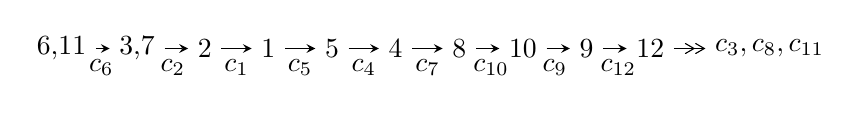
\begin{tikzpicture}[x=23pt, y=7pt]
	% node
	\node (A0) at (-1/8, 0) {6,11};
	\node (A1) at (17/16, 0) {3,7};
	\node (A2) at (17/8, 0) {2};
	\node (A3) at (25/8, 0) {1};
	\node (A4) at (33/8, 0) {5};
	\node (A5) at (41/8, 0) {4};
	\node (A6) at (49/8, 0) {8};
	\node (A7) at (57/8, 0) {10};
	\node (A8) at (65/8, 0) {9};
	\node (A9) at (73/8, 0) {12};
	\node (C1) at (1/2, -1) {$c_{6}$};
	\node (C2) at (13/8, -1) {$c_{2}$};
	\node (C3) at (21/8, -1) {$c_{1}$};
	\node (C4) at (29/8, -1) {$c_{5}$};
	\node (C5) at (37/8, -1) {$c_{4}$};
	\node (C6) at (45/8, -1) {$c_{7}$};
	\node (C7) at (53/8, -1) {$c_{10}$};
	\node (C8) at (61/8, -1) {$c_{9}$};
	\node (C9) at (69/8, -1) {$c_{12}$};
	\node (A10) at (11, 0) {$c_{3},c_{8},c_{11}$};

	% edge
	\draw[->,>=stealth]	
	(A0) edge (A1) (A1) edge (A2) (A2) edge (A3) (A3) edge (A4) (A4) edge (A5) (A5) edge (A6) (A6) edge (A7) (A7) edge (A8) (A8) edge (A9) ;
	\draw[->>,>={angle 60}]	
	(A9) edge (A10);
\end{tikzpicture} \\ 

\end{tabular} \\

\footnotetext{
The image of knot diagram is generated by the software ``\textbf{Draw programme}" developed by Andrew Bartholomew(\url{http://www.layer8.co.uk/maths/draw/index.htm\#Running-draw}), where we modified some parts for our purpose(\url{https://github.com/CATsTAILs/LinksPainter}).
}\phantom \\ \newline 
\centering \textbf{Ideals for irreducible components\footnotemark of $X_{\text{par}}$} 
 
\begin{align*}
I^u_{1}&=\langle 
-8.97013\times10^{55} u^{29}-1.58329\times10^{56} u^{28}+\cdots+4.35231\times10^{58} b+6.55011\times10^{57},\\
\phantom{I^u_{1}}&\phantom{= \langle  }3.18509\times10^{57} u^{29}-1.03463\times10^{58} u^{28}+\cdots+1.82362\times10^{61} a+1.17215\times10^{61},\\
\phantom{I^u_{1}}&\phantom{= \langle  }u^{30}+2 u^{29}+\cdots+100 u-419\rangle \\
I^u_{2}&=\langle 
-5 u^{12}+21 u^{10}-7 u^9-18 u^8+33 u^7-17 u^6-26 u^5+26 u^4+7 u^3-15 u^2+2 b+3 u+5,\\
\phantom{I^u_{2}}&\phantom{= \langle  }11 u^{12}+2 u^{11}-48 u^{10}+6 u^9+49 u^8-64 u^7+21 u^6+72 u^5-53 u^4-32 u^3+37 u^2+2 a- u-14,\\
\phantom{I^u_{2}}&\phantom{= \langle  }u^{13}+u^{12}-4 u^{11}-3 u^{10}+4 u^9-2 u^8-2 u^7+7 u^6+u^5-6 u^4+2 u^2- u-1\rangle \\
\\
\end{align*}
\raggedright * 2 irreducible components of $\dim_{\mathbb{C}}=0$, with total 43 representations.\\
\footnotetext{All coefficients of polynomials are rational numbers. But the coefficients are sometimes approximated in decimal forms when there is not enough margin.}
\newpage
\renewcommand{\arraystretch}{1}
\centering \section*{I. $I^u_{1}= \langle -8.97\times10^{55} u^{29}-1.58\times10^{56} u^{28}+\cdots+4.35\times10^{58} b+6.55\times10^{57},\;3.19\times10^{57} u^{29}-1.03\times10^{58} u^{28}+\cdots+1.82\times10^{61} a+1.17\times10^{61},\;u^{30}+2 u^{29}+\cdots+100 u-419 \rangle$}
\flushleft \textbf{(i) Arc colorings}\\
\begin{tabular}{m{7pt} m{180pt} m{7pt} m{180pt} }
\flushright $a_{6}=$&$\begin{pmatrix}1\\0\end{pmatrix}$ \\
\flushright $a_{11}=$&$\begin{pmatrix}0\\u\end{pmatrix}$ \\
\flushright $a_{3}=$&$\begin{pmatrix}-0.000174658 u^{29}+0.000567352 u^{28}+\cdots+1.47843 u-0.642763\\0.00206100 u^{29}+0.00363781 u^{28}+\cdots-0.596168 u-0.150497\end{pmatrix}$ \\
\flushright $a_{7}=$&$\begin{pmatrix}1\\- u^2\end{pmatrix}$ \\
\flushright $a_{2}=$&$\begin{pmatrix}0.00188635 u^{29}+0.00420517 u^{28}+\cdots+0.882267 u-0.793260\\0.00206100 u^{29}+0.00363781 u^{28}+\cdots-0.596168 u-0.150497\end{pmatrix}$ \\
\flushright $a_{1}=$&$\begin{pmatrix}0.00358201 u^{29}+0.00533243 u^{28}+\cdots-0.845448 u+0.146579\\-0.00430260 u^{29}-0.00434093 u^{28}+\cdots+2.70318 u-1.08487\end{pmatrix}$ \\
\flushright $a_{5}=$&$\begin{pmatrix}0.0000550185 u^{29}+0.00136950 u^{28}+\cdots+0.855142 u-0.322525\\-0.000908531 u^{29}+0.0000579815 u^{28}+\cdots+0.0808855 u-1.03300\end{pmatrix}$ \\
\flushright $a_{4}=$&$\begin{pmatrix}0.000107308 u^{29}+0.000594620 u^{28}+\cdots+0.877150 u+0.182757\\0.0000965840 u^{29}+0.00130720 u^{28}+\cdots-0.0289697 u-0.664503\end{pmatrix}$ \\
\flushright $a_{8}=$&$\begin{pmatrix}-0.0000748679 u^{29}+0.000914934 u^{28}+\cdots+0.654950 u+0.759505\\-0.00255893 u^{29}-0.00377164 u^{28}+\cdots+0.375116 u-0.944810\end{pmatrix}$ \\
\flushright $a_{10}=$&$\begin{pmatrix}- u\\u\end{pmatrix}$ \\
\flushright $a_{9}=$&$\begin{pmatrix}-0.0000732909 u^{29}-0.00133981 u^{28}+\cdots-1.16207 u-0.158293\\0.00125946 u^{29}+0.00337516 u^{28}+\cdots-0.328027 u+0.0230528\end{pmatrix}$ \\
\flushright $a_{12}=$&$\begin{pmatrix}0.00156530 u^{29}+0.00377669 u^{28}+\cdots-0.300258 u-0.872709\\-0.00228589 u^{29}-0.00278519 u^{28}+\cdots+2.15799 u-0.0655795\end{pmatrix}$\\&\end{tabular}
\flushleft \textbf{(ii) Obstruction class $= -1$}\\~\\
\flushleft \textbf{(iii) Cusp Shapes $= 0.000964221 u^{29}+0.00738326 u^{28}+\cdots+11.2158 u+0.582373$}\\~\\
\newpage\renewcommand{\arraystretch}{1}
\flushleft \textbf{(iv) u-Polynomials at the component}\newline \\
\begin{tabular}{m{50pt}|m{274pt}}
Crossings & \hspace{64pt}u-Polynomials at each crossing \\
\hline $$\begin{aligned}c_{1}\end{aligned}$$&$\begin{aligned}
&u^{30}+54 u^{29}+\cdots+35644 u+961
\end{aligned}$\\
\hline $$\begin{aligned}c_{2},c_{5}\end{aligned}$$&$\begin{aligned}
&u^{30}+2 u^{29}+\cdots+274 u+31
\end{aligned}$\\
\hline $$\begin{aligned}c_{3},c_{9}\end{aligned}$$&$\begin{aligned}
&u^{30}- u^{29}+\cdots-18 u-9
\end{aligned}$\\
\hline $$\begin{aligned}c_{4},c_{7}\end{aligned}$$&$\begin{aligned}
&u^{30}+7 u^{29}+\cdots-58 u+7
\end{aligned}$\\
\hline $$\begin{aligned}c_{6},c_{10}\end{aligned}$$&$\begin{aligned}
&u^{30}+2 u^{29}+\cdots+100 u-419
\end{aligned}$\\
\hline $$\begin{aligned}c_{8},c_{11}\end{aligned}$$&$\begin{aligned}
&u^{30}- u^{29}+\cdots- u-1
\end{aligned}$\\
\hline $$\begin{aligned}c_{12}\end{aligned}$$&$\begin{aligned}
&u^{30}+3 u^{29}+\cdots+276288 u-31624
\end{aligned}$\\
\hline
\end{tabular}\\~\\
\newpage\renewcommand{\arraystretch}{1}
\flushleft \textbf{(v) Riley Polynomials at the component}\newline \\
\begin{tabular}{m{50pt}|m{274pt}}
Crossings & \hspace{64pt}Riley Polynomials at each crossing \\
\hline $$\begin{aligned}c_{1}\end{aligned}$$&$\begin{aligned}
&y^{30}-166 y^{29}+\cdots+2665988060 y+923521
\end{aligned}$\\
\hline $$\begin{aligned}c_{2},c_{5}\end{aligned}$$&$\begin{aligned}
&y^{30}-54 y^{29}+\cdots-35644 y+961
\end{aligned}$\\
\hline $$\begin{aligned}c_{3},c_{9}\end{aligned}$$&$\begin{aligned}
&y^{30}+47 y^{29}+\cdots+972 y+81
\end{aligned}$\\
\hline $$\begin{aligned}c_{4},c_{7}\end{aligned}$$&$\begin{aligned}
&y^{30}+23 y^{29}+\cdots-1614 y+49
\end{aligned}$\\
\hline $$\begin{aligned}c_{6},c_{10}\end{aligned}$$&$\begin{aligned}
&y^{30}+10 y^{29}+\cdots+590846 y+175561
\end{aligned}$\\
\hline $$\begin{aligned}c_{8},c_{11}\end{aligned}$$&$\begin{aligned}
&y^{30}-21 y^{29}+\cdots-19 y+1
\end{aligned}$\\
\hline $$\begin{aligned}c_{12}\end{aligned}$$&$\begin{aligned}
&y^{30}+121 y^{29}+\cdots+1307553376 y+1000077376
\end{aligned}$\\
\hline
\end{tabular}\\~\\
\newpage\flushleft \textbf{(vi) Complex Volumes and Cusp Shapes}
$$\begin{array}{c|c|c}  
\text{Solutions to }I^u_{1}& \I (\text{vol} + \sqrt{-1}CS) & \text{Cusp shape}\\
 \hline 
\begin{aligned}
u &= \phantom{-}0.642590 + 0.700606 I \\
a &= \phantom{-}0.106716 - 1.072760 I \\
b &= -0.347246 + 1.044670 I\end{aligned}
 & \phantom{-}0.82927 + 4.60566 I & \phantom{-}7.38656 - 8.01596 I \\ \hline\begin{aligned}
u &= \phantom{-}0.642590 - 0.700606 I \\
a &= \phantom{-}0.106716 + 1.072760 I \\
b &= -0.347246 - 1.044670 I\end{aligned}
 & \phantom{-}0.82927 - 4.60566 I & \phantom{-}7.38656 + 8.01596 I \\ \hline\begin{aligned}
u &= -0.814116 + 0.677327 I \\
a &= \phantom{-}0.504066 + 1.067370 I \\
b &= -0.549219 - 0.145896 I\end{aligned}
 & -0.77900 - 2.06540 I & \phantom{-}3.22171 + 2.38317 I \\ \hline\begin{aligned}
u &= -0.814116 - 0.677327 I \\
a &= \phantom{-}0.504066 - 1.067370 I \\
b &= -0.549219 + 0.145896 I\end{aligned}
 & -0.77900 + 2.06540 I & \phantom{-}3.22171 - 2.38317 I \\ \hline\begin{aligned}
u &= \phantom{-}0.560922 + 0.747663 I \\
a &= \phantom{-}0.472626 - 0.864157 I \\
b &= -0.104866 + 0.109501 I\end{aligned}
 & \phantom{-}0.327633 - 0.843648 I & \phantom{-}6.72873 + 1.86017 I \\ \hline\begin{aligned}
u &= \phantom{-}0.560922 - 0.747663 I \\
a &= \phantom{-}0.472626 + 0.864157 I \\
b &= -0.104866 - 0.109501 I\end{aligned}
 & \phantom{-}0.327633 + 0.843648 I & \phantom{-}6.72873 - 1.86017 I \\ \hline\begin{aligned}
u &= -0.055990 + 1.128490 I \\
a &= -0.924318 + 0.178825 I \\
b &= \phantom{-}2.41962 - 0.23089 I\end{aligned}
 & -10.40080 + 1.46441 I & -1.99581 - 5.01569 I \\ \hline\begin{aligned}
u &= -0.055990 - 1.128490 I \\
a &= -0.924318 - 0.178825 I \\
b &= \phantom{-}2.41962 + 0.23089 I\end{aligned}
 & -10.40080 - 1.46441 I & -1.99581 + 5.01569 I \\ \hline\begin{aligned}
u &= -0.586638 + 0.553835 I \\
a &= \phantom{-}0.155793 + 1.119640 I \\
b &= -0.651578 - 0.537140 I\end{aligned}
 & -1.29989 - 1.54235 I & \phantom{-}1.52237 + 4.53495 I \\ \hline\begin{aligned}
u &= -0.586638 - 0.553835 I \\
a &= \phantom{-}0.155793 - 1.119640 I \\
b &= -0.651578 + 0.537140 I\end{aligned}
 & -1.29989 + 1.54235 I & \phantom{-}1.52237 - 4.53495 I\\
 \hline 
 \end{array}$$\newpage$$\begin{array}{c|c|c}  
\text{Solutions to }I^u_{1}& \I (\text{vol} + \sqrt{-1}CS) & \text{Cusp shape}\\
 \hline 
\begin{aligned}
u &= \phantom{-}1.307100 + 0.036349 I \\
a &= \phantom{-}0.71975 + 1.63357 I \\
b &= -0.798397 - 0.708430 I\end{aligned}
 & \phantom{-}3.26183 - 2.73720 I & \phantom{-}10.18982 + 2.92398 I \\ \hline\begin{aligned}
u &= \phantom{-}1.307100 - 0.036349 I \\
a &= \phantom{-}0.71975 - 1.63357 I \\
b &= -0.798397 + 0.708430 I\end{aligned}
 & \phantom{-}3.26183 + 2.73720 I & \phantom{-}10.18982 - 2.92398 I \\ \hline\begin{aligned}
u &= -0.049314 + 1.329620 I \\
a &= -0.356304 + 0.123824 I \\
b &= \phantom{-}1.85890 - 0.07524 I\end{aligned}
 & -11.24640 - 1.91319 I & \phantom{-}0.75047 + 3.50106 I \\ \hline\begin{aligned}
u &= -0.049314 - 1.329620 I \\
a &= -0.356304 - 0.123824 I \\
b &= \phantom{-}1.85890 + 0.07524 I\end{aligned}
 & -11.24640 + 1.91319 I & \phantom{-}0.75047 - 3.50106 I \\ \hline\begin{aligned}
u &= \phantom{-}0.403283 + 1.277970 I \\
a &= -0.507314 - 0.949307 I \\
b &= \phantom{-}1.40638 + 0.97678 I\end{aligned}
 & -3.40270 - 3.64668 I & \phantom{-}2.86245 + 2.46962 I \\ \hline\begin{aligned}
u &= \phantom{-}0.403283 - 1.277970 I \\
a &= -0.507314 + 0.949307 I \\
b &= \phantom{-}1.40638 - 0.97678 I\end{aligned}
 & -3.40270 + 3.64668 I & \phantom{-}2.86245 - 2.46962 I \\ \hline\begin{aligned}
u &= -0.276632 + 1.333170 I \\
a &= -0.334409 + 0.791751 I \\
b &= \phantom{-}1.39749 - 0.61314 I\end{aligned}
 & -7.55076 - 1.32763 I & -0.010757 + 0.862501 I \\ \hline\begin{aligned}
u &= -0.276632 - 1.333170 I \\
a &= -0.334409 - 0.791751 I \\
b &= \phantom{-}1.39749 + 0.61314 I\end{aligned}
 & -7.55076 + 1.32763 I & -0.010757 - 0.862501 I \\ \hline\begin{aligned}
u &= -0.309884 + 0.543530 I \\
a &= -0.220039 + 0.852834 I \\
b &= -0.933653 - 0.345827 I\end{aligned}
 & -1.56864 - 1.53975 I & \phantom{-}1.10369 + 4.69285 I \\ \hline\begin{aligned}
u &= -0.309884 - 0.543530 I \\
a &= -0.220039 - 0.852834 I \\
b &= -0.933653 + 0.345827 I\end{aligned}
 & -1.56864 + 1.53975 I & \phantom{-}1.10369 - 4.69285 I\\
 \hline 
 \end{array}$$\newpage$$\begin{array}{c|c|c}  
\text{Solutions to }I^u_{1}& \I (\text{vol} + \sqrt{-1}CS) & \text{Cusp shape}\\
 \hline 
\begin{aligned}
u &= \phantom{-}0.242225 + 1.368910 I \\
a &= -0.111633 - 0.819227 I \\
b &= \phantom{-}1.153510 + 0.418732 I\end{aligned}
 & -4.09460 + 6.61711 I & \phantom{-}2.97271 - 4.66549 I \\ \hline\begin{aligned}
u &= \phantom{-}0.242225 - 1.368910 I \\
a &= -0.111633 + 0.819227 I \\
b &= \phantom{-}1.153510 - 0.418732 I\end{aligned}
 & -4.09460 - 6.61711 I & \phantom{-}2.97271 + 4.66549 I \\ \hline\begin{aligned}
u &= \phantom{-}0.531314\phantom{ +0.000000I} \\
a &= \phantom{-}0.442861\phantom{ +0.000000I} \\
b &= \phantom{-}0.183744\phantom{ +0.000000I}\end{aligned}
 & \phantom{-}0.719441\phantom{ +0.000000I} & \phantom{-}14.3760\phantom{ +0.000000I} \\ \hline\begin{aligned}
u &= -1.55692\phantom{ +0.000000I} \\
a &= -0.621196\phantom{ +0.000000I} \\
b &= \phantom{-}0.986893\phantom{ +0.000000I}\end{aligned}
 & \phantom{-}7.16181\phantom{ +0.000000I} & \phantom{-}20.2020\phantom{ +0.000000I} \\ \hline\begin{aligned}
u &= -1.34575 + 1.55021 I \\
a &= \phantom{-}1.43706 + 0.93333 I \\
b &= -2.22516 - 0.41486 I\end{aligned}
 & -15.4447 - 11.8067 I & \phantom{-}3.77024 + 5.11220 I \\ \hline\begin{aligned}
u &= -1.34575 - 1.55021 I \\
a &= \phantom{-}1.43706 - 0.93333 I \\
b &= -2.22516 + 0.41486 I\end{aligned}
 & -15.4447 + 11.8067 I & \phantom{-}3.77024 - 5.11220 I \\ \hline\begin{aligned}
u &= \phantom{-}1.48358 + 1.48152 I \\
a &= \phantom{-}1.42930 - 1.02156 I \\
b &= -2.15106 + 0.44424 I\end{aligned}
 & -19.4159 + 5.5271 I & \phantom{-}1.12565 - 2.12056 I \\ \hline\begin{aligned}
u &= \phantom{-}1.48358 - 1.48152 I \\
a &= \phantom{-}1.42930 + 1.02156 I \\
b &= -2.15106 - 0.44424 I\end{aligned}
 & -19.4159 - 5.5271 I & \phantom{-}1.12565 + 2.12056 I \\ \hline\begin{aligned}
u &= -1.68857 + 1.42229 I \\
a &= \phantom{-}1.44579 + 1.14500 I \\
b &= -2.06005 - 0.54414 I\end{aligned}
 & -14.5803 + 0.6531 I & \phantom{-}6.00000 + 0. I\phantom{ +0.000000I} \\ \hline\begin{aligned}
u &= -1.68857 - 1.42229 I \\
a &= \phantom{-}1.44579 - 1.14500 I \\
b &= -2.06005 + 0.54414 I\end{aligned}
 & -14.5803 - 0.6531 I & \phantom{-}6.00000 + 0. I\phantom{ +0.000000I}\\
 \hline 
 \end{array}$$\newpage\newpage\renewcommand{\arraystretch}{1}
\centering \section*{II. $I^u_{2}= \langle -5 u^{12}+21 u^{10}+\cdots+2 b+5,\;11 u^{12}+2 u^{11}+\cdots+2 a-14,\;u^{13}+u^{12}+\cdots- u-1 \rangle$}
\flushleft \textbf{(i) Arc colorings}\\
\begin{tabular}{m{7pt} m{180pt} m{7pt} m{180pt} }
\flushright $a_{6}=$&$\begin{pmatrix}1\\0\end{pmatrix}$ \\
\flushright $a_{11}=$&$\begin{pmatrix}0\\u\end{pmatrix}$ \\
\flushright $a_{3}=$&$\begin{pmatrix}-\frac{11}{2} u^{12}- u^{11}+\cdots+\frac{1}{2} u+7\\\frac{5}{2} u^{12}-\frac{21}{2} u^{10}+\cdots-\frac{3}{2} u-\frac{5}{2}\end{pmatrix}$ \\
\flushright $a_{7}=$&$\begin{pmatrix}1\\- u^2\end{pmatrix}$ \\
\flushright $a_{2}=$&$\begin{pmatrix}-3 u^{12}- u^{11}+\cdots- u+\frac{9}{2}\\\frac{5}{2} u^{12}-\frac{21}{2} u^{10}+\cdots-\frac{3}{2} u-\frac{5}{2}\end{pmatrix}$ \\
\flushright $a_{1}=$&$\begin{pmatrix}-\frac{3}{2} u^{12}-2 u^{11}+\cdots-\frac{3}{2} u+5\\\frac{3}{2} u^{12}+\frac{1}{2} u^{11}+\cdots-2 u-\frac{3}{2}\end{pmatrix}$ \\
\flushright $a_{5}=$&$\begin{pmatrix}2 u^{12}+u^{11}+\cdots- u-\frac{3}{2}\\\frac{5}{2} u^{12}+\frac{1}{2} u^{11}+\cdots+\frac{17}{2} u^2-\frac{7}{2}\end{pmatrix}$ \\
\flushright $a_{4}=$&$\begin{pmatrix}- u^{12}+5 u^{10}- u^9-7 u^8+6 u^7-9 u^5+6 u^4+7 u^3-6 u^2-2 u+3\\3 u^{12}+u^{11}+\cdots+u-\frac{11}{2}\end{pmatrix}$ \\
\flushright $a_{8}=$&$\begin{pmatrix}-\frac{11}{2} u^{12}- u^{11}+\cdots+\frac{3}{2} u+\frac{9}{2}\\3 u^{12}-\frac{1}{2} u^{11}+\cdots+6 u^2-\frac{5}{2} u\end{pmatrix}$ \\
\flushright $a_{10}=$&$\begin{pmatrix}- u\\u\end{pmatrix}$ \\
\flushright $a_{9}=$&$\begin{pmatrix}-\frac{1}{2} u^{12}+\frac{3}{2} u^{11}+\cdots+4 u-2\\- u^{12}-\frac{1}{2} u^{11}+\cdots+\frac{1}{2} u+2\end{pmatrix}$ \\
\flushright $a_{12}=$&$\begin{pmatrix}-4 u^{12}-2 u^{11}+\cdots-14 u^2+\frac{13}{2}\\4 u^{12}+\frac{1}{2} u^{11}+\cdots-\frac{7}{2} u-3\end{pmatrix}$\\&\end{tabular}
\flushleft \textbf{(ii) Obstruction class $= 1$}\\~\\
\flushleft \textbf{(iii) Cusp Shapes $= 3 u^{12}-4 u^{11}-\frac{21}{2} u^{10}+\frac{39}{2} u^9-\frac{7}{2} u^8-\frac{51}{2} u^7+42 u^6-15 u^5-\frac{41}{2} u^4+\frac{41}{2} u^3-3 u^2-12 u+\frac{21}{2}$}\\~\\
\newpage\renewcommand{\arraystretch}{1}
\flushleft \textbf{(iv) u-Polynomials at the component}\newline \\
\begin{tabular}{m{50pt}|m{274pt}}
Crossings & \hspace{64pt}u-Polynomials at each crossing \\
\hline $$\begin{aligned}c_{1}\end{aligned}$$&$\begin{aligned}
&u^{13}-13 u^{12}+\cdots+7 u-1
\end{aligned}$\\
\hline $$\begin{aligned}c_{2}\end{aligned}$$&$\begin{aligned}
&u^{13}+3 u^{12}+\cdots-3 u-1
\end{aligned}$\\
\hline $$\begin{aligned}c_{3}\end{aligned}$$&$\begin{aligned}
&u^{13}+8 u^{11}+\cdots+3 u+1
\end{aligned}$\\
\hline $$\begin{aligned}c_{4}\end{aligned}$$&$\begin{aligned}
&u^{13}+2 u^{11}+\cdots+3 u+1
\end{aligned}$\\
\hline $$\begin{aligned}c_{5}\end{aligned}$$&$\begin{aligned}
&u^{13}-3 u^{12}+\cdots-3 u+1
\end{aligned}$\\
\hline $$\begin{aligned}c_{6}\end{aligned}$$&$\begin{aligned}
&u^{13}+u^{12}+\cdots- u-1
\end{aligned}$\\
\hline $$\begin{aligned}c_{7}\end{aligned}$$&$\begin{aligned}
&u^{13}+2 u^{11}+\cdots+3 u-1
\end{aligned}$\\
\hline $$\begin{aligned}c_{8}\end{aligned}$$&$\begin{aligned}
&u^{13}-6 u^{11}+\cdots-2 u-3
\end{aligned}$\\
\hline $$\begin{aligned}c_{9}\end{aligned}$$&$\begin{aligned}
&u^{13}+8 u^{11}+\cdots+3 u-1
\end{aligned}$\\
\hline $$\begin{aligned}c_{10}\end{aligned}$$&$\begin{aligned}
&u^{13}- u^{12}+\cdots- u+1
\end{aligned}$\\
\hline $$\begin{aligned}c_{11}\end{aligned}$$&$\begin{aligned}
&u^{13}-6 u^{11}+\cdots-2 u+3
\end{aligned}$\\
\hline $$\begin{aligned}c_{12}\end{aligned}$$&$\begin{aligned}
&u^{13}-2 u^{12}+\cdots-13 u+1
\end{aligned}$\\
\hline
\end{tabular}\\~\\
\newpage\renewcommand{\arraystretch}{1}
\flushleft \textbf{(v) Riley Polynomials at the component}\newline \\
\begin{tabular}{m{50pt}|m{274pt}}
Crossings & \hspace{64pt}Riley Polynomials at each crossing \\
\hline $$\begin{aligned}c_{1}\end{aligned}$$&$\begin{aligned}
&y^{13}-37 y^{12}+\cdots+11 y-1
\end{aligned}$\\
\hline $$\begin{aligned}c_{2},c_{5}\end{aligned}$$&$\begin{aligned}
&y^{13}-13 y^{12}+\cdots+7 y-1
\end{aligned}$\\
\hline $$\begin{aligned}c_{3},c_{9}\end{aligned}$$&$\begin{aligned}
&y^{13}+16 y^{12}+\cdots-5 y-1
\end{aligned}$\\
\hline $$\begin{aligned}c_{4},c_{7}\end{aligned}$$&$\begin{aligned}
&y^{13}+4 y^{12}+\cdots+y-1
\end{aligned}$\\
\hline $$\begin{aligned}c_{6},c_{10}\end{aligned}$$&$\begin{aligned}
&y^{13}-9 y^{12}+\cdots+5 y-1
\end{aligned}$\\
\hline $$\begin{aligned}c_{8},c_{11}\end{aligned}$$&$\begin{aligned}
&y^{13}-12 y^{12}+\cdots+46 y-9
\end{aligned}$\\
\hline $$\begin{aligned}c_{12}\end{aligned}$$&$\begin{aligned}
&y^{13}+30 y^{12}+\cdots+25 y-1
\end{aligned}$\\
\hline
\end{tabular}\\~\\
\newpage\flushleft \textbf{(vi) Complex Volumes and Cusp Shapes}
$$\begin{array}{c|c|c}  
\text{Solutions to }I^u_{2}& \I (\text{vol} + \sqrt{-1}CS) & \text{Cusp shape}\\
 \hline 
\begin{aligned}
u &= \phantom{-}0.954573 + 0.260088 I \\
a &= -0.92363 - 1.20575 I \\
b &= \phantom{-}0.582097 - 0.018888 I\end{aligned}
 & -3.98060 + 1.00568 I & \phantom{-}1.162112 - 0.615451 I \\ \hline\begin{aligned}
u &= \phantom{-}0.954573 - 0.260088 I \\
a &= -0.92363 + 1.20575 I \\
b &= \phantom{-}0.582097 + 0.018888 I\end{aligned}
 & -3.98060 - 1.00568 I & \phantom{-}1.162112 + 0.615451 I \\ \hline\begin{aligned}
u &= \phantom{-}0.266976 + 1.054200 I \\
a &= -0.532456 + 0.412592 I \\
b &= \phantom{-}2.10432 - 0.01987 I\end{aligned}
 & -9.61091 - 1.01135 I & \phantom{-}7.06702 - 0.15470 I \\ \hline\begin{aligned}
u &= \phantom{-}0.266976 - 1.054200 I \\
a &= -0.532456 - 0.412592 I \\
b &= \phantom{-}2.10432 + 0.01987 I\end{aligned}
 & -9.61091 + 1.01135 I & \phantom{-}7.06702 + 0.15470 I \\ \hline\begin{aligned}
u &= -0.752928 + 0.297393 I \\
a &= \phantom{-}1.030040 + 0.709707 I \\
b &= -0.921610 - 0.177058 I\end{aligned}
 & -0.796848 - 0.470467 I & \phantom{-}2.94539 - 1.34493 I \\ \hline\begin{aligned}
u &= -0.752928 - 0.297393 I \\
a &= \phantom{-}1.030040 - 0.709707 I \\
b &= -0.921610 + 0.177058 I\end{aligned}
 & -0.796848 + 0.470467 I & \phantom{-}2.94539 + 1.34493 I \\ \hline\begin{aligned}
u &= -0.684151 + 0.344382 I \\
a &= -1.27505 + 0.67741 I \\
b &= \phantom{-}0.314319 + 0.549467 I\end{aligned}
 & -1.36517 - 5.98644 I & \phantom{-}4.94299 + 5.64527 I \\ \hline\begin{aligned}
u &= -0.684151 - 0.344382 I \\
a &= -1.27505 - 0.67741 I \\
b &= \phantom{-}0.314319 - 0.549467 I\end{aligned}
 & -1.36517 + 5.98644 I & \phantom{-}4.94299 - 5.64527 I \\ \hline\begin{aligned}
u &= \phantom{-}0.460968 + 0.533555 I \\
a &= \phantom{-}0.56985 - 1.90658 I \\
b &= -0.813036 + 0.713273 I\end{aligned}
 & \phantom{-}0.43653 + 3.26322 I & \phantom{-}5.30243 - 3.80898 I \\ \hline\begin{aligned}
u &= \phantom{-}0.460968 - 0.533555 I \\
a &= \phantom{-}0.56985 + 1.90658 I \\
b &= -0.813036 - 0.713273 I\end{aligned}
 & \phantom{-}0.43653 - 3.26322 I & \phantom{-}5.30243 + 3.80898 I\\
 \hline 
 \end{array}$$\newpage$$\begin{array}{c|c|c}  
\text{Solutions to }I^u_{2}& \I (\text{vol} + \sqrt{-1}CS) & \text{Cusp shape}\\
 \hline 
\begin{aligned}
u &= -1.60034 + 0.28645 I \\
a &= -0.84754 + 1.61343 I \\
b &= \phantom{-}0.858896 - 0.743211 I\end{aligned}
 & \phantom{-}2.06490 + 2.83942 I & \phantom{-}2.96766 - 2.65257 I \\ \hline\begin{aligned}
u &= -1.60034 - 0.28645 I \\
a &= -0.84754 - 1.61343 I \\
b &= \phantom{-}0.858896 + 0.743211 I\end{aligned}
 & \phantom{-}2.06490 - 2.83942 I & \phantom{-}2.96766 + 2.65257 I \\ \hline\begin{aligned}
u &= \phantom{-}1.70981\phantom{ +0.000000I} \\
a &= \phantom{-}0.957563\phantom{ +0.000000I} \\
b &= -1.24998\phantom{ +0.000000I}\end{aligned}
 & \phantom{-}6.76499\phantom{ +0.000000I} & -0.775210\phantom{ +0.000000I}\\
 \hline 
 \end{array}$$\newpage
\newpage\renewcommand{\arraystretch}{1}
\centering \section*{ III. u-Polynomials}
\begin{tabular}{m{50pt}|m{274pt}}
Crossings & \hspace{64pt}u-Polynomials at each crossing \\
\hline $$\begin{aligned}c_{1}\end{aligned}$$&$\begin{aligned}
&(u^{13}-13 u^{12}+\cdots+7 u-1)(u^{30}+54 u^{29}+\cdots+35644 u+961)
\end{aligned}$\\
\hline $$\begin{aligned}c_{2}\end{aligned}$$&$\begin{aligned}
&(u^{13}+3 u^{12}+\cdots-3 u-1)(u^{30}+2 u^{29}+\cdots+274 u+31)
\end{aligned}$\\
\hline $$\begin{aligned}c_{3}\end{aligned}$$&$\begin{aligned}
&(u^{13}+8 u^{11}+\cdots+3 u+1)(u^{30}- u^{29}+\cdots-18 u-9)
\end{aligned}$\\
\hline $$\begin{aligned}c_{4}\end{aligned}$$&$\begin{aligned}
&(u^{13}+2 u^{11}+\cdots+3 u+1)(u^{30}+7 u^{29}+\cdots-58 u+7)
\end{aligned}$\\
\hline $$\begin{aligned}c_{5}\end{aligned}$$&$\begin{aligned}
&(u^{13}-3 u^{12}+\cdots-3 u+1)(u^{30}+2 u^{29}+\cdots+274 u+31)
\end{aligned}$\\
\hline $$\begin{aligned}c_{6}\end{aligned}$$&$\begin{aligned}
&(u^{13}+u^{12}+\cdots- u-1)(u^{30}+2 u^{29}+\cdots+100 u-419)
\end{aligned}$\\
\hline $$\begin{aligned}c_{7}\end{aligned}$$&$\begin{aligned}
&(u^{13}+2 u^{11}+\cdots+3 u-1)(u^{30}+7 u^{29}+\cdots-58 u+7)
\end{aligned}$\\
\hline $$\begin{aligned}c_{8}\end{aligned}$$&$\begin{aligned}
&(u^{13}-6 u^{11}+\cdots-2 u-3)(u^{30}- u^{29}+\cdots- u-1)
\end{aligned}$\\
\hline $$\begin{aligned}c_{9}\end{aligned}$$&$\begin{aligned}
&(u^{13}+8 u^{11}+\cdots+3 u-1)(u^{30}- u^{29}+\cdots-18 u-9)
\end{aligned}$\\
\hline $$\begin{aligned}c_{10}\end{aligned}$$&$\begin{aligned}
&(u^{13}- u^{12}+\cdots- u+1)(u^{30}+2 u^{29}+\cdots+100 u-419)
\end{aligned}$\\
\hline $$\begin{aligned}c_{11}\end{aligned}$$&$\begin{aligned}
&(u^{13}-6 u^{11}+\cdots-2 u+3)(u^{30}- u^{29}+\cdots- u-1)
\end{aligned}$\\
\hline $$\begin{aligned}c_{12}\end{aligned}$$&$\begin{aligned}
&(u^{13}-2 u^{12}+\cdots-13 u+1)(u^{30}+3 u^{29}+\cdots+276288 u-31624)
\end{aligned}$\\
\hline
\end{tabular}\newpage\renewcommand{\arraystretch}{1}
\centering \section*{ IV. Riley Polynomials}
\begin{tabular}{m{50pt}|m{274pt}}
Crossings & \hspace{64pt}Riley Polynomials at each crossing \\
\hline $$\begin{aligned}c_{1}\end{aligned}$$&$\begin{aligned}
&(y^{13}-37 y^{12}+\cdots+11 y-1)\\
&\cdot(y^{30}-166 y^{29}+\cdots+2665988060 y+923521)
\end{aligned}$\\
\hline $$\begin{aligned}c_{2},c_{5}\end{aligned}$$&$\begin{aligned}
&(y^{13}-13 y^{12}+\cdots+7 y-1)(y^{30}-54 y^{29}+\cdots-35644 y+961)
\end{aligned}$\\
\hline $$\begin{aligned}c_{3},c_{9}\end{aligned}$$&$\begin{aligned}
&(y^{13}+16 y^{12}+\cdots-5 y-1)(y^{30}+47 y^{29}+\cdots+972 y+81)
\end{aligned}$\\
\hline $$\begin{aligned}c_{4},c_{7}\end{aligned}$$&$\begin{aligned}
&(y^{13}+4 y^{12}+\cdots+y-1)(y^{30}+23 y^{29}+\cdots-1614 y+49)
\end{aligned}$\\
\hline $$\begin{aligned}c_{6},c_{10}\end{aligned}$$&$\begin{aligned}
&(y^{13}-9 y^{12}+\cdots+5 y-1)(y^{30}+10 y^{29}+\cdots+590846 y+175561)
\end{aligned}$\\
\hline $$\begin{aligned}c_{8},c_{11}\end{aligned}$$&$\begin{aligned}
&(y^{13}-12 y^{12}+\cdots+46 y-9)(y^{30}-21 y^{29}+\cdots-19 y+1)
\end{aligned}$\\
\hline $$\begin{aligned}c_{12}\end{aligned}$$&$\begin{aligned}
&(y^{13}+30 y^{12}+\cdots+25 y-1)\\
&\cdot(y^{30}+121 y^{29}+\cdots+1307553376 y+1000077376)
\end{aligned}$\\
\hline
\end{tabular}
\vskip 2pc
\end{document}